\chapter{Set up dell'applicazione web}
In questo capitolo vengono introdotti i software che permetteranno di configurare  l'applicazione web realizzata affinché sia online.

\section{Hosting}
L'hosting è un servizio che permetta di caricare dei contenuti su un server web affinché sia accessibile dalla rete internet.
Si utilizza un Hosting di Amazon (a pagamento) che è una macchina virtuale dove vi è installato \textbf{Bitnami} (web server), e vi tutti gli strumenti necessari per procedere al setup.

\section{Database}
Si procede alla creazione del database sul nostro host, è necessario quindi connettersi al modulo PhpMyAdmin dell'hosting.

\subsection{Putty Setup}
Per effettuare il setup dell'applicativo Putty si devono effettuare i seguenti passaggi:
\begin{enumerate}
\item installare il Client SSH per la gestione in remoto di sistemi informatici \textbf{Putty};
\item aprire Putty;
\item nella sezione \textbf{Session}, nel campo \textbf{Host Name} inserire l'indirizzo IP del nostro hosting;
\item selezionare la porta 80;
\item entrare sezione \textbf{Connection};
\item entrare nella sotto sezione \textbf{SSH};
\item selezionare la voce \textbf{Auth};
\item nella sezione \textbf{Authentication Parameters} trovare la voce \textbf{Private key File for Authentication}, cliccare Sfoglia/Browse e selezionare il file di autenticazione fornitoci (\textit{LightEC2private.ppk});
\item sempre nella sotto sezione SSH selezionare la voce \textbf{Tunnels};
\item settare la \textbf{Source Port} con \textbf{8888};
\item settare \textbf{Destination};
\item cliccare Aggiungi/Add;
\item assicurarsi che la porta aggiunta sia tra le \textbf{Forwarded Ports};
\item cliccare \textbf{Apri/Open} per aprire la connessione SSH con il server. La sessione SSH includerà ora un tunnel SSH sicuro tra le due porte specificate;
\item inserire come username \textbf{bitnami};
\end{enumerate}

\begin{figure}[h]
	\centering
	\caption{Connessione stabilita con successo}
	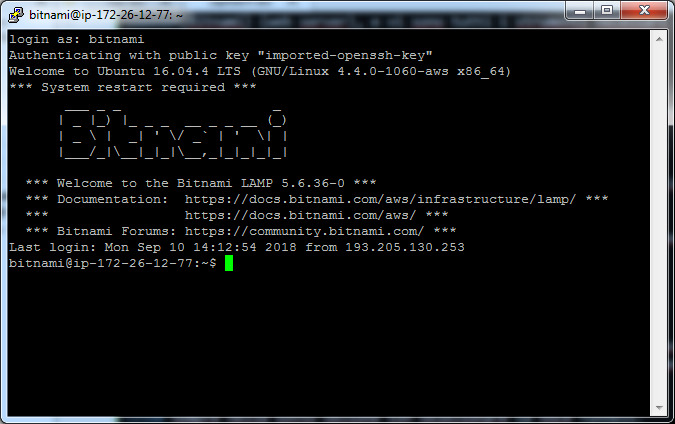
\includegraphics[width= 15cm]{bitnami.png}
\end{figure}
Lasciando il terminale aperto si prosegue con la connessione a phpmyadmin.
\subsubsection{Connessione a PhpMyAdmin}
Per connettersi a questo modulo si procede come segue:
\begin{enumerate}
\item si apre il web browser;
\item si naviga all'indirizzo \textbf{http://127.0.0.1:8888/phpmyadmin/};
\item si apre il pannello di login di phpmyadmin come in figura:
\begin{figure}[h]
	\centering
	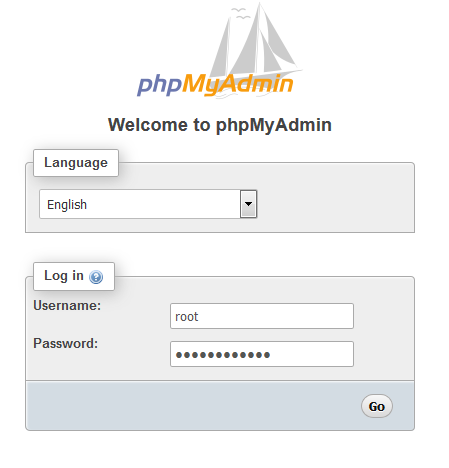
\includegraphics[width= 13cm]{phpmyadmin.png}
\end{figure}


\item si immettono le credenziali - Username : \textbf{root} -Password;
\item si clicca \textbf{Go} per entrare nel pannello di PhpMyAdmin;
\end{enumerate}
\newpage
Entrati nel pannello si procede alla creazione del database, cliccando sulla voce new dalla \textbf{tree-view} sulla sinistra. Fare riferimento alla seguente immagine.
\begin{figure}[h]
	\centering
	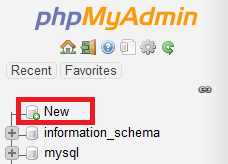
\includegraphics[]{create_database.png}
\end{figure}

Ora si procede come segue:
\begin{enumerate}
\item Inserire il nome del database (\textbf{orto\_botanico}).
\item Selezionare il set di caratteri \textbf{utf8\_general\_ci}.
\item Premere il bottone \textbf{Create}.
\item Selezionare dalla tree-view il database \textbf{orto\_botanico}.
\item Cliccare la Tab \textbf{SQL}.
\item Creare le tabelle definite una per una nella sezione \textbf{3.1.3}. Le tabelle devono rispettare il seguente ordine a causa delle dipendenze da chiavi esterne:
\begin{itemize}
\item \textbf{photo};
\item \textbf{beacon};
\item \textbf{species};
\item \textbf{phenological\_phase};
\item \textbf{place};
\item \textbf{plant};
\item \textbf{exists\_table};
\item \textbf{visitors};
\item \textbf{advice};
\end{itemize}
\end{enumerate}
A questo punto è possibile iniziare a inserire i dati nel database. 
\newpage
\subsection{geojson.io}
Per comodità per la \textbf{latitudine} e \textbf{longitudine} di un elemento e per il \textbf{boundary} di un orto botanico si utilizza il sito web \textbf{http://geojson.io}. Ecco un esempio di utilizzo:

\begin{figure}[h]
	\centering
	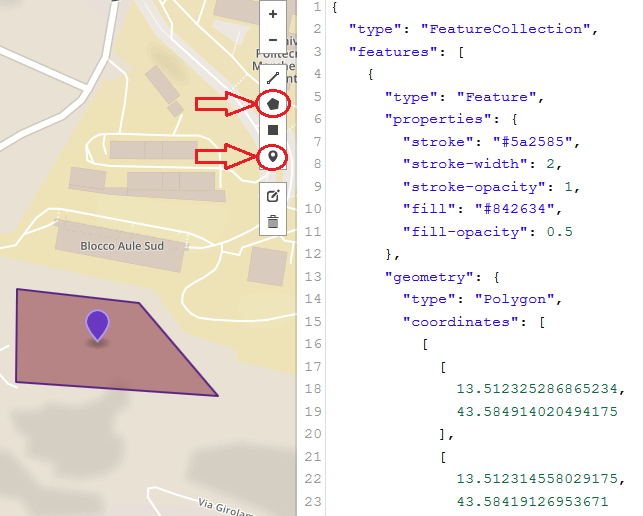
\includegraphics[scale=0.9]{geojson.png}
\end{figure}

Come è possibile vedere dall'immagine, sulla destra troviamo il codice che poi sarà inserito nella colonna \textbf{boundary}. Sul riquadro della mappa invece, sulla destra si trova una sidebar volta a creare vari elementi. Quelli cerchiati sono quelli di interesse, utilizzati nel progetto. \newline 
Inoltre cliccando sull'elemento creato nella mappa è possibile specificare ulteriori parametri come suggeriscono le seguenti immagini.

\begin{figure}[H]
	\centering
	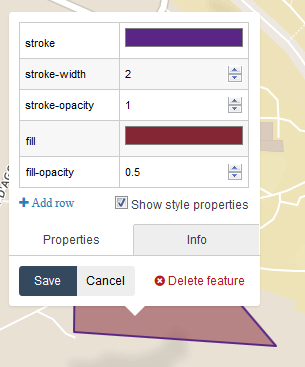
\includegraphics[]{place1.png}
	\caption{Click sul poligono : possibilità di specificare attributi grafici come il colore, la linea di contorno e l'opacità.}
\end{figure}

\begin{figure}[H]
	\centering
	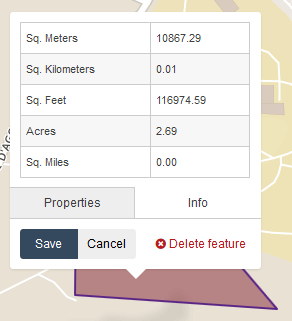
\includegraphics[]{place2.png}
	\caption{Click sul poligono : informazioni utili.}
\end{figure}

\begin{figure}[H]
	\centering
	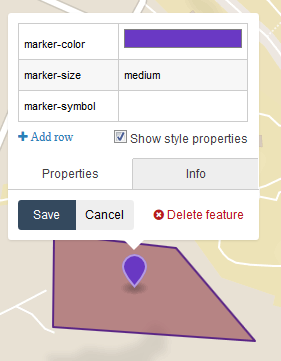
\includegraphics[]{beacon1.png}
	\caption{Click sul beacon : possibilità di specificare attributi grafici come il colore, il simbolo e la dimensione.}
\end{figure}

\begin{figure}[H]
	\centering
	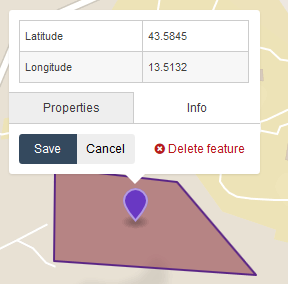
\includegraphics[]{beacon2.png}
	\caption{Click sul beacon : latitudine e longitudine.}
\end{figure}

\section{Caricamento Files con WinSCP}
WinSCP, acronimo di Windows Secure Copy che è un client SFTP e FTP di tipo grafico che ha come funzione principale quella di trasferimento dati tra un computer locale ed uno remoto. In più WinSCP consente semplici funzionalità di file manager. Per trasferimenti sicuri usa Secure Shell (SSH) e supporta il protocollo SCP in aggiunta al SFTP \cite{sito_winscp}.  \newline
Per configurare la connessione e effettuare il caricamento dei file si procede come segue:
\begin{enumerate}
\item si Installa WinSCP;
\item si avvia il client WinSCRP;
\item si imposta l'indirizzo IP;
\item si imposta come username \textbf{bitnami};
\item si clicca su \textbf{Advanced}, a questo punto si apre una finestra;
\item cliccare la sezione \textbf{SSH};
\item aprire la voce \textbf{Authentication};
\item immettere la chiave \textit{LightEC2private.ppk} sul campo \textbf{Private Key File};
\item sfogliare le directory del server fino a raggiungere \textbf{/opt/bitnami/apache2/htdocs};
\item trascinare i files desiderati ricordando di applicare le modifiche al file config.php che sviluppando in locale ha parametri differenti;
\end{enumerate}

\section{Disabilitare il modulo Pagespeed}
Per evitare eventuali problemi di visualizzazione delle icone dei beacon sulla mappa, è necessario disabilitare il modulo pagespeed.
Per fare ciò bisogna localizzare il file \textbf{pagespeed.conf} che è situato nella directory \textbf{/opt/bitnami/apache2/conf}, aprire il file e modificare la linea \textbf{ModPagespeed on} in \textbf{ModPagespeed off}. 
Infine è necessario riavviare il servizio di apache con il comando \textbf{service httpd restart}.


\newpage

\section{Permessi per uploads}
Per far funzionare correttamente gli script php di upload e non incorrerre errori particolari è necessario dare tutti i permessi alle seguenti cartelle:
\begin{itemize}
\item /opt/bitnami/php/tmp
\item /opt/bitnami/apache2/htdocs/images
\end{itemize}
Questa operazione può essere effettuata tramite terminale con i seguenti passaggi:
\begin{enumerate}
\item Ci si assicura che la connessione SSH sia aperta.
\item Si ottengono i permessi di amministratore utilizzando il comando \textbf{sudo su}.
\item Si esegue l'istruzione chmod 755 -R /opt/bitnami/php/tmp per i permessi della cartella temp.
\item Si esegue l'istruzione chmod 755 -R /opt/bitnami/apache2/htdocs/images per i permessi della cartella images.
\end{enumerate}
In alternativa è possibile utilizzare \textbf{WinSCP} : cliccando su proprietà è possibile impostare i permessi come in figura.
\begin{figure}[H]
	\centering
	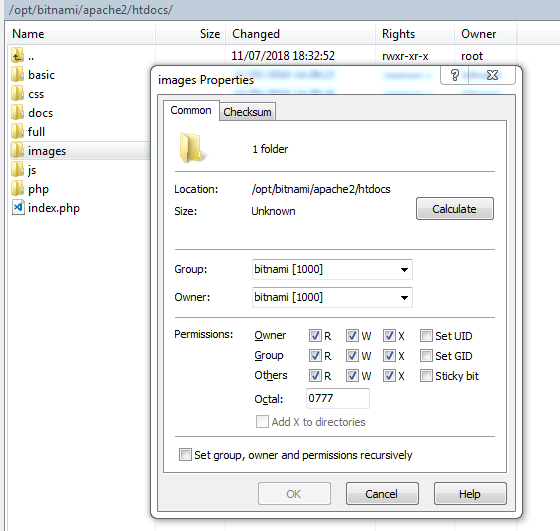
\includegraphics[scale=0.7]{permission.png}
	\caption{Proprietà : Assicurarsi che Write sia spuntato}
\end{figure}

\section{Accesso all'applicazione Web con il protocollo HTTPS}
Per accedere da desktop all'applicazione web utilizzando il protocollo sicuro è necessario aggiungere un'eccezione al certificato che è \textbf{self-signed}. \newline
\begin{figure}[H]
	\centering
	\caption{Aggiungendo l'eccezione è possibile navigare nel sito utilizzando a pieno le API}
	\label{fig:firefox_https}
	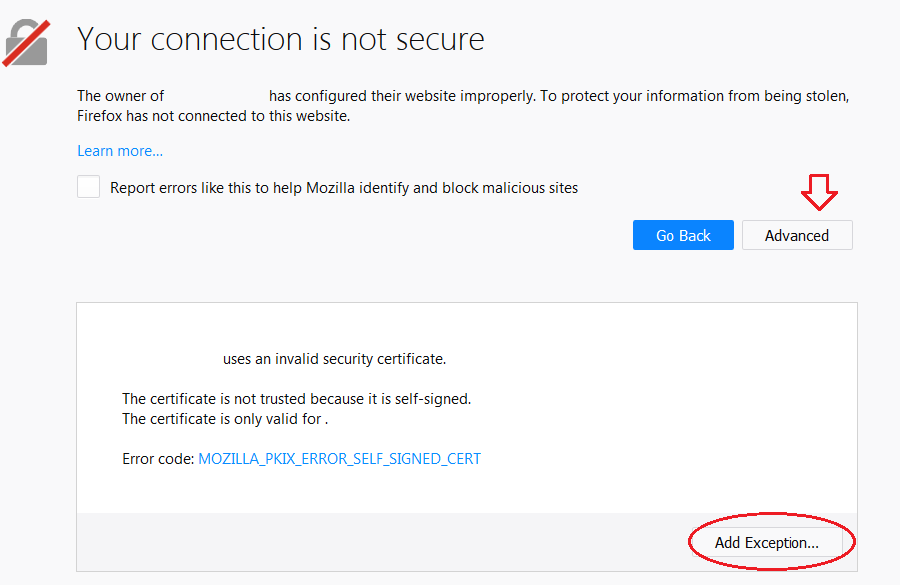
\includegraphics[scale=0.6]{firefox_https.png}
\end{figure} 

\begin{figure}[H]
	\centering
	\caption{Confermando l'eccezione sarà possibile la navigazione}
	\label{fig:exception}
	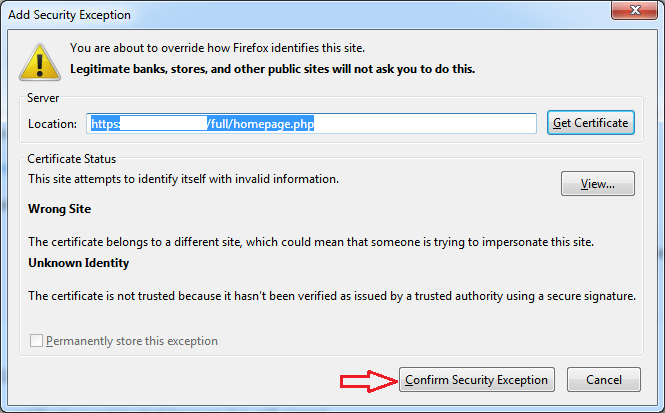
\includegraphics[scale=0.6]{exception.png}
\end{figure} 

\begin{figure}[H]
	\centering
	\caption{Richiesta di Localizzazione da Desktop}
	\label{fig:geolocation_desktop}
	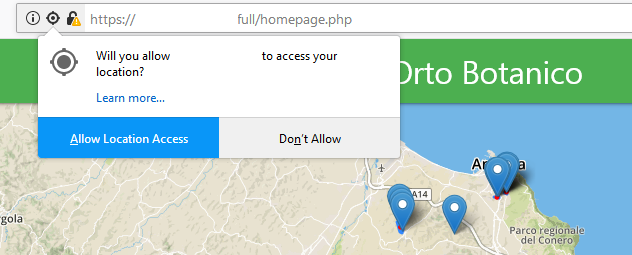
\includegraphics[scale=0.6]{geolocation_desktop.png}
\end{figure} 

\newpage

\section{Gestione del Database tramite script manage.php}
Dopo aver eseguito tutte le configurazioni precedentemente introdotte, tramite la pagina manage.php non si ha più necessità di utilizzare il modulo PhpMyAdmin per manipolare i dati nel database. \newline
Ora verranno introdotte le funzioni restanti messe a disposizione da questo script che non sono state introdotte in precedenza.
\begin{itemize}
\item modifica del nome di una tabella, cliccando semplicemente sul nome;
\item notifica tooltip del tipo della colonna, lasciando il puntatore (evento \textbf{onhover}) sopra il nome della colonna;
\item modifica del tipo della colonna, cliccando sopra il nome della colonna;
\item modifica del nome della colonna, cliccando sulla cella, sulla parte esterna del nome;
\end{itemize}
Si ricordano inoltre le funzioni già introdotte, quali:
\begin{itemize}
\item modifica dei valori di un record;
\item inserimento di un record facilitato tramite utilizzo di menù a tendina già formattati con i dati idonei (es: possibili valori di una enumerazione o di una chiave esterna);
\item eliminazione di un record;
\end{itemize}




